\documentclass[a4paper,11pt,openany]{book}
\usepackage[utf8]{inputenc}
\usepackage[left=2.54cm,top=2.54cm,right=2.54cm,bottom=2.54cm]{geometry}
\usepackage[spanish]{babel}
\usepackage{amsmath}
\usepackage{amsfonts}
\usepackage{amssymb}
\usepackage{graphicx}
\usepackage{color}
\usepackage[usenames,dvipsnames]{xcolor}
\usepackage{pifont}
\usepackage{marvosym}
\newtheorem{teo}{Teorema}
\newtheorem{ejemplo}{Ejemplo}
\newtheorem{defi}{Definición}
\newtheorem{coro}{Corolario}
\newtheorem{prueba}{Prueba}
\newtheorem{exmp}{Example}[section]
\newtheorem{ejer}{Ejercicio}[section]
\def\proof{\paragraph{\textsf{Demostración.} }}
\def\endproof{\hfill $\blacksquare$ \\}
\usepackage{multirow, array} % para las tablas
\usepackage{multirow}
\usepackage{tabularx}
\usepackage{float} % para usar [H]
\usepackage{tikz}
\usepackage[all]{xy}
\usepackage{cancel}
\usetikzlibrary{positioning}
\usepackage{enumitem}
\newcommand*{\itembolasazules}[1]{% bolas 3D
\footnotesize\protect\tikz[baseline=-3pt]%
\protect\node[scale=.7, circle, shade, ball
color=green]{\color{white}\Large\bf#1};}
\usepackage{tcolorbox} 
\tcbuselibrary{listingsutf8}
\newtcolorbox[auto counter,number within=section]{example}[2][]
{colback=green!5!white,colframe=green!75!black,fonttitle=\bfseries, title=Ejercicio~\thetcbcounter: #2,#1}
\usepackage{background}
\backgroundsetup{
placement=center,
angle=0,
scale=1.1,
contents= {{
\includegraphics{HojaCuadriculada.png}}}
}

\begin{document}
\begin{titlepage}
 
\begin{center}
\vspace*{-1in}
\begin{figure}[htb]
\begin{center}

\includegraphics[width=7cm]{ETITC.png}
\end{center}
\end{figure}

{\sc \huge Escuela Tecnológica Instituto Técnico Central (ETITC)}\\
\vspace*{0.15in}
Facultad de sistemas\\
\vspace*{0.6in}
\begin{Large}
\textbf{Taller 4 : Funciones, Límites y Derivadas en los Complejos} \\
\textbf{Matem{\'a}ticas Especiales}\\
\end{Large}
\vspace*{0.3in}
\begin{large}
{\bf Autores} \\
 
\ 
 
Sergio Alejandro Enrrique Caballero Leon\\ 
Johan Alejandro Sogamoso Camacho \\
David Andrés Valero Vanegas \\
\end{large}
\vspace*{0.3in}
 
\end{center}
 
\begin{center}
{\bf Presentado a:} \\
 
\ 
 
Carlos Romero \\
 
\
 
Bogot{\'a}, Octubre de 2022.
\end{center}
 
\end{titlepage}

\newpage

\definecolor{ao(english)}{rgb}{0.0, 0.5, 0.0}

\graphicspath{ {images/} }

\begin{center}
\textbf{Funciones}
\end{center}

En los ejercicio \textbf{(\,1\,)} al \textbf{(\,5\,)} sea $f(z)$ la función que que actúa sobre el conjunto dado $\mathnormal{S}$. Hallar la imágen $\mathnormal{S\,'}$ correspondiente a cada conjunto y graficar su respectivo mapeo.\\

\textcolor{ao(english)}{(\,1\,)} $\mathnormal{S}$ es $\boxed{\bf{y\,=\,1\,-\,x}}$ y $\boxed{\bf{f(z)\,=\,z\,+\,i\,(i\,-\,2)}}$.

\definecolor{ao}{rgb}{0.0, 0.0, 1.0}

$$\underbrace{y\,=\,1\,-\,x}_{E_{1}}$$

\textcolor{ao(english)}{\ding{46}} Sustituir $z\,=\,x\,+\,i\,y$ en $f(z)$.

$$f(x\,+\,i\,y)\,=\,x\,+\,i\,y\,+\,i\,(i\,-\,2)\,=\,x\,+\,i\,y\,+\,\underbrace{i^{2}}_{-\,1}\,-\,2\,i\,=\,x\,+\,i\,y\,-\,1\,-\,2\,i$$

$$w\,=\,\underbrace{(x\,-\,1)}_{u(x\,,\,y)}\,+\,i\,\underbrace{(y\,-\,2)}_{v(x\,,\,y)}$$

$$\underbrace{u\,=\,x\,-\,1}_{E_{2}} \qquad;\qquad \underbrace{v\,=\,y\,-\,2}_{E_{3}}$$

\textcolor{ao(english)}{\ding{46}} Despejar $x$ en $E_{1}$.

$$y\,=\,1\,-\,x \quad\iff\quad \underbrace{x\,=\,1\,-\,y}_{E_{4}}$$

\textcolor{ao(english)}{\ding{46}} Sustituir $E_{4}$ en $E_{2}$.

$$u\,=\,\textcolor{ao}{1\,-\,y}\,-\,1 \quad\iff\quad \underbrace{u\,=\,-\,y}_{E_{5}}$$

\textcolor{ao(english)}{\ding{46}} Despejar $y$ en $E_{5}$.

$$u\,=\,-\,y \quad\iff\quad \underbrace{y\,=\,-\,u}_{E_{6}}$$

\textcolor{ao(english)}{\ding{46}} Sustituir $E_{6}$ en $E_{3}$.

$$v\,=\,\textcolor{ao}{-\,u}\,-\,2$$

\textcolor{ao(english)}{\ding{46}} Mapeo z-plano.

\begin{center}
     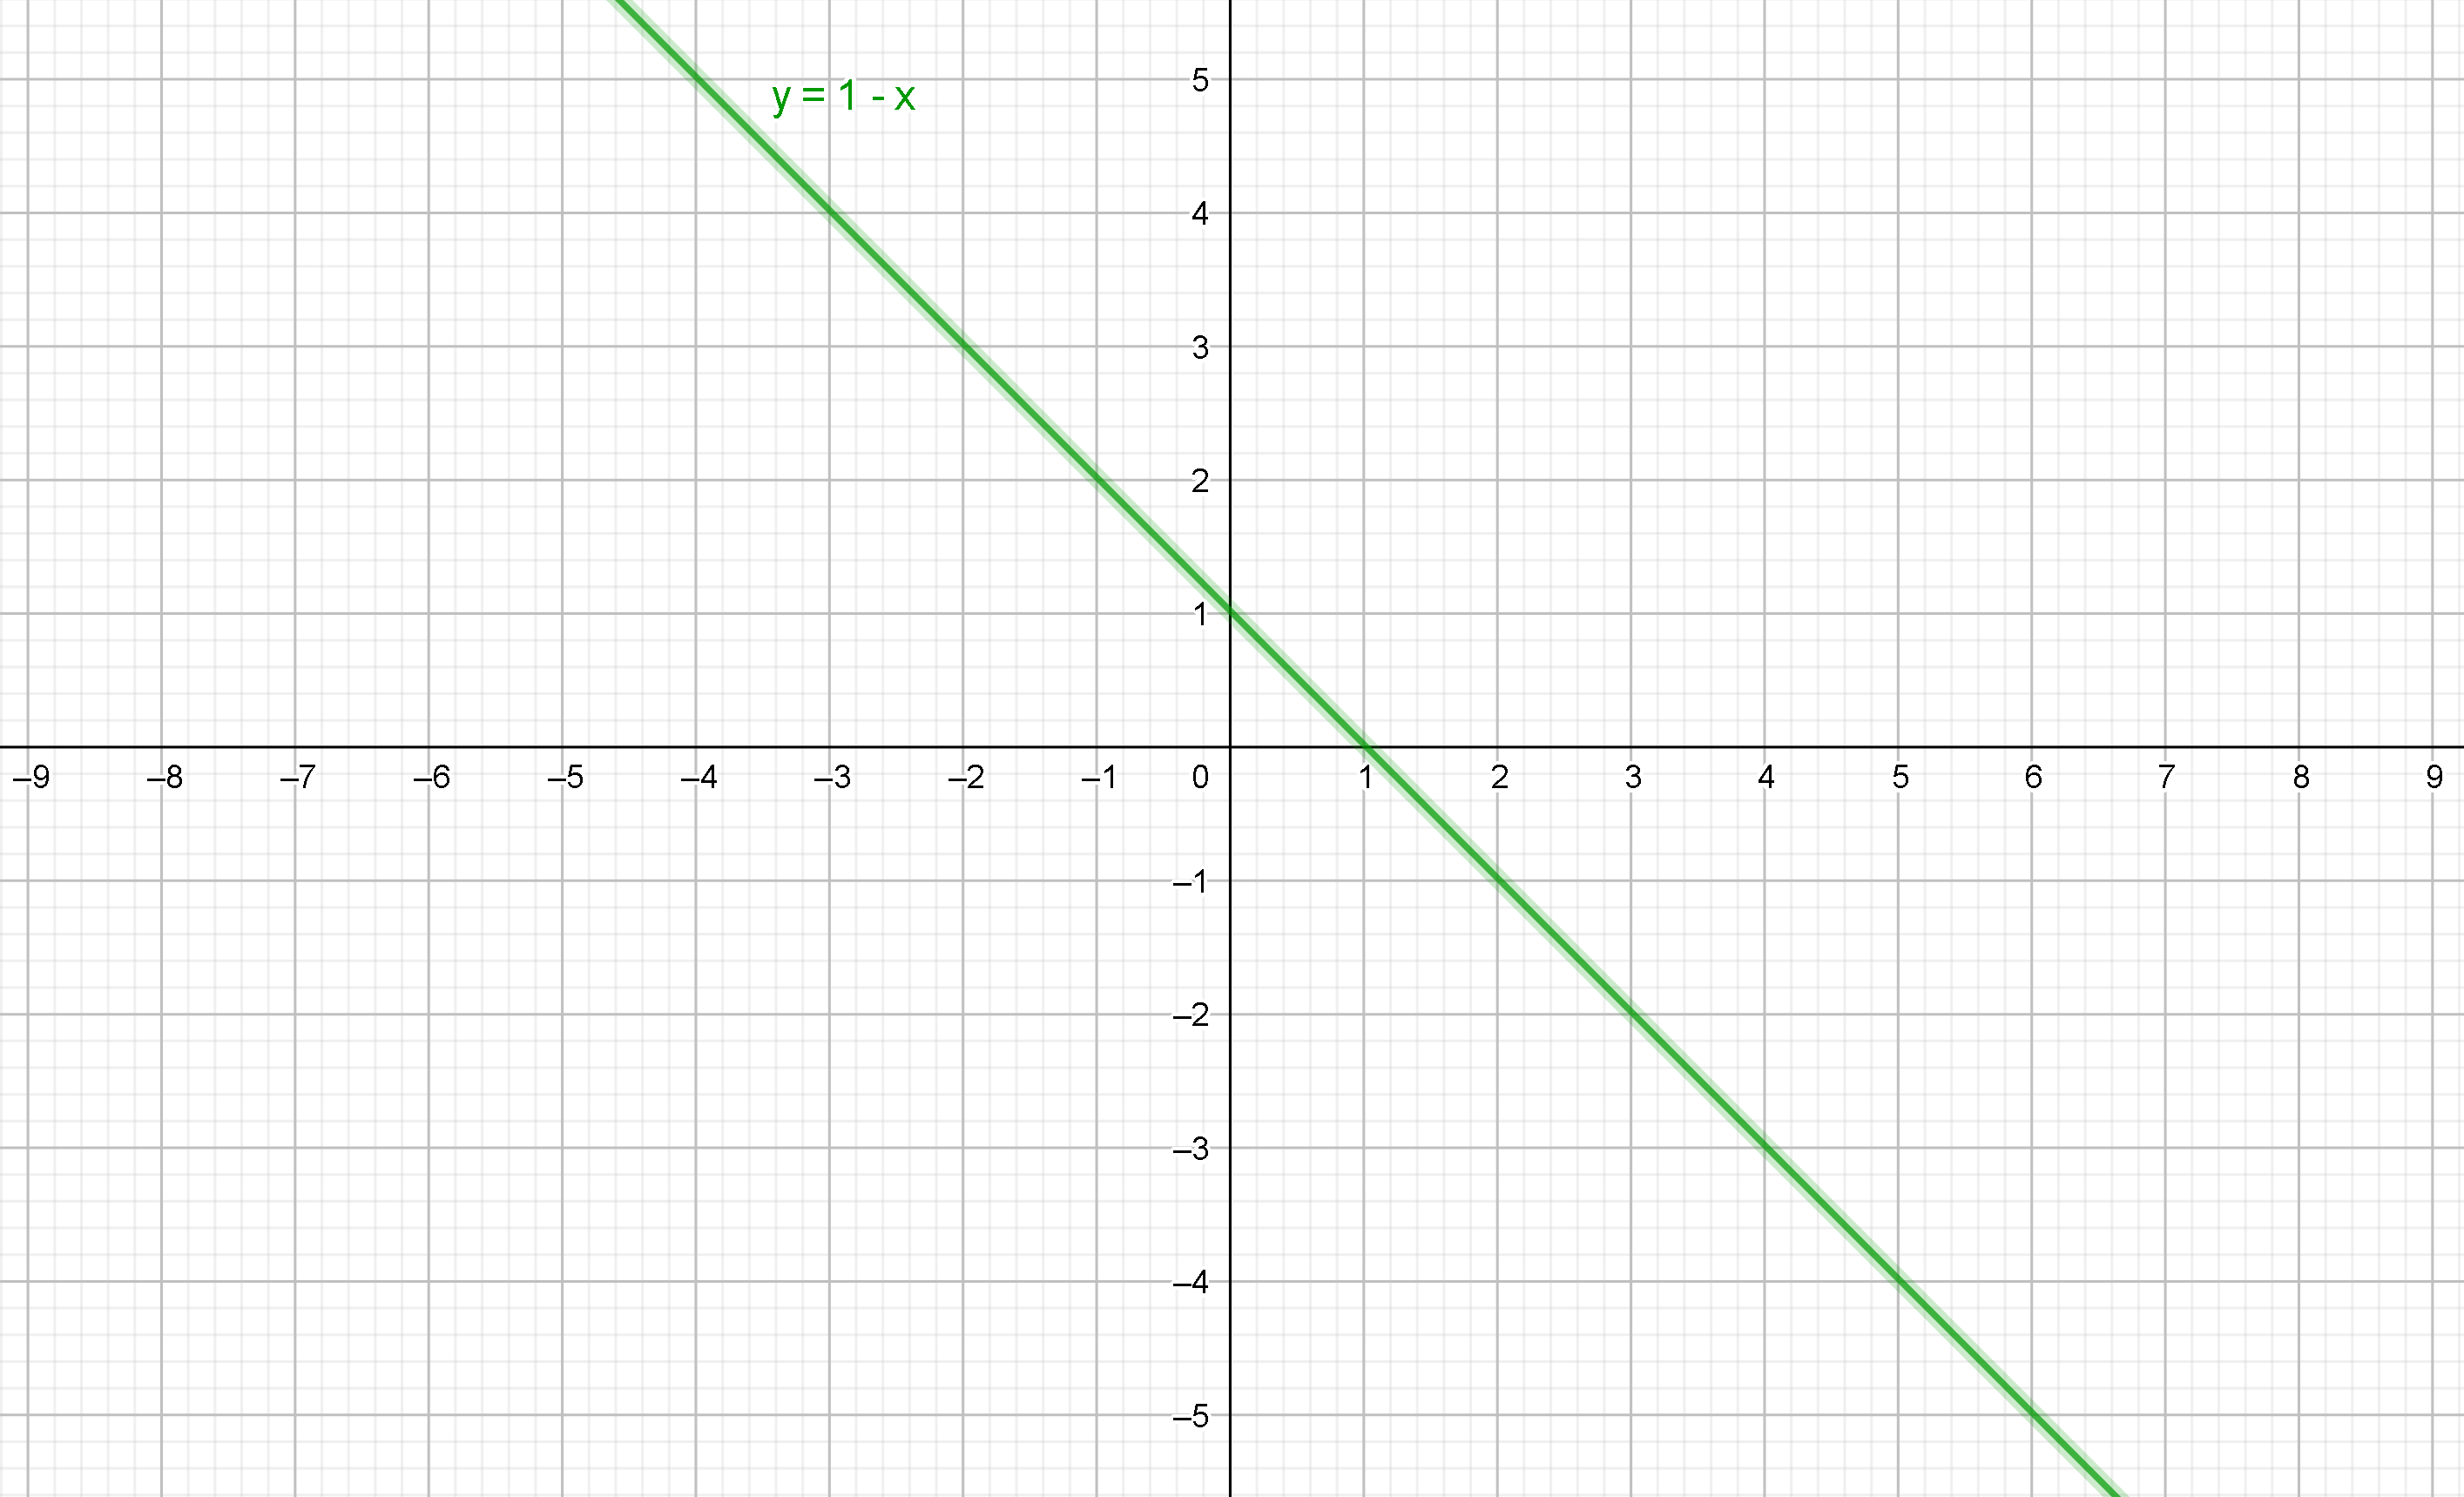
\includegraphics[width=11cm]{Mapeo Ej 1 z.png}
\end{center}

\textcolor{ao(english)}{\ding{46}} Mapeo w-plano.

\begin{center}
     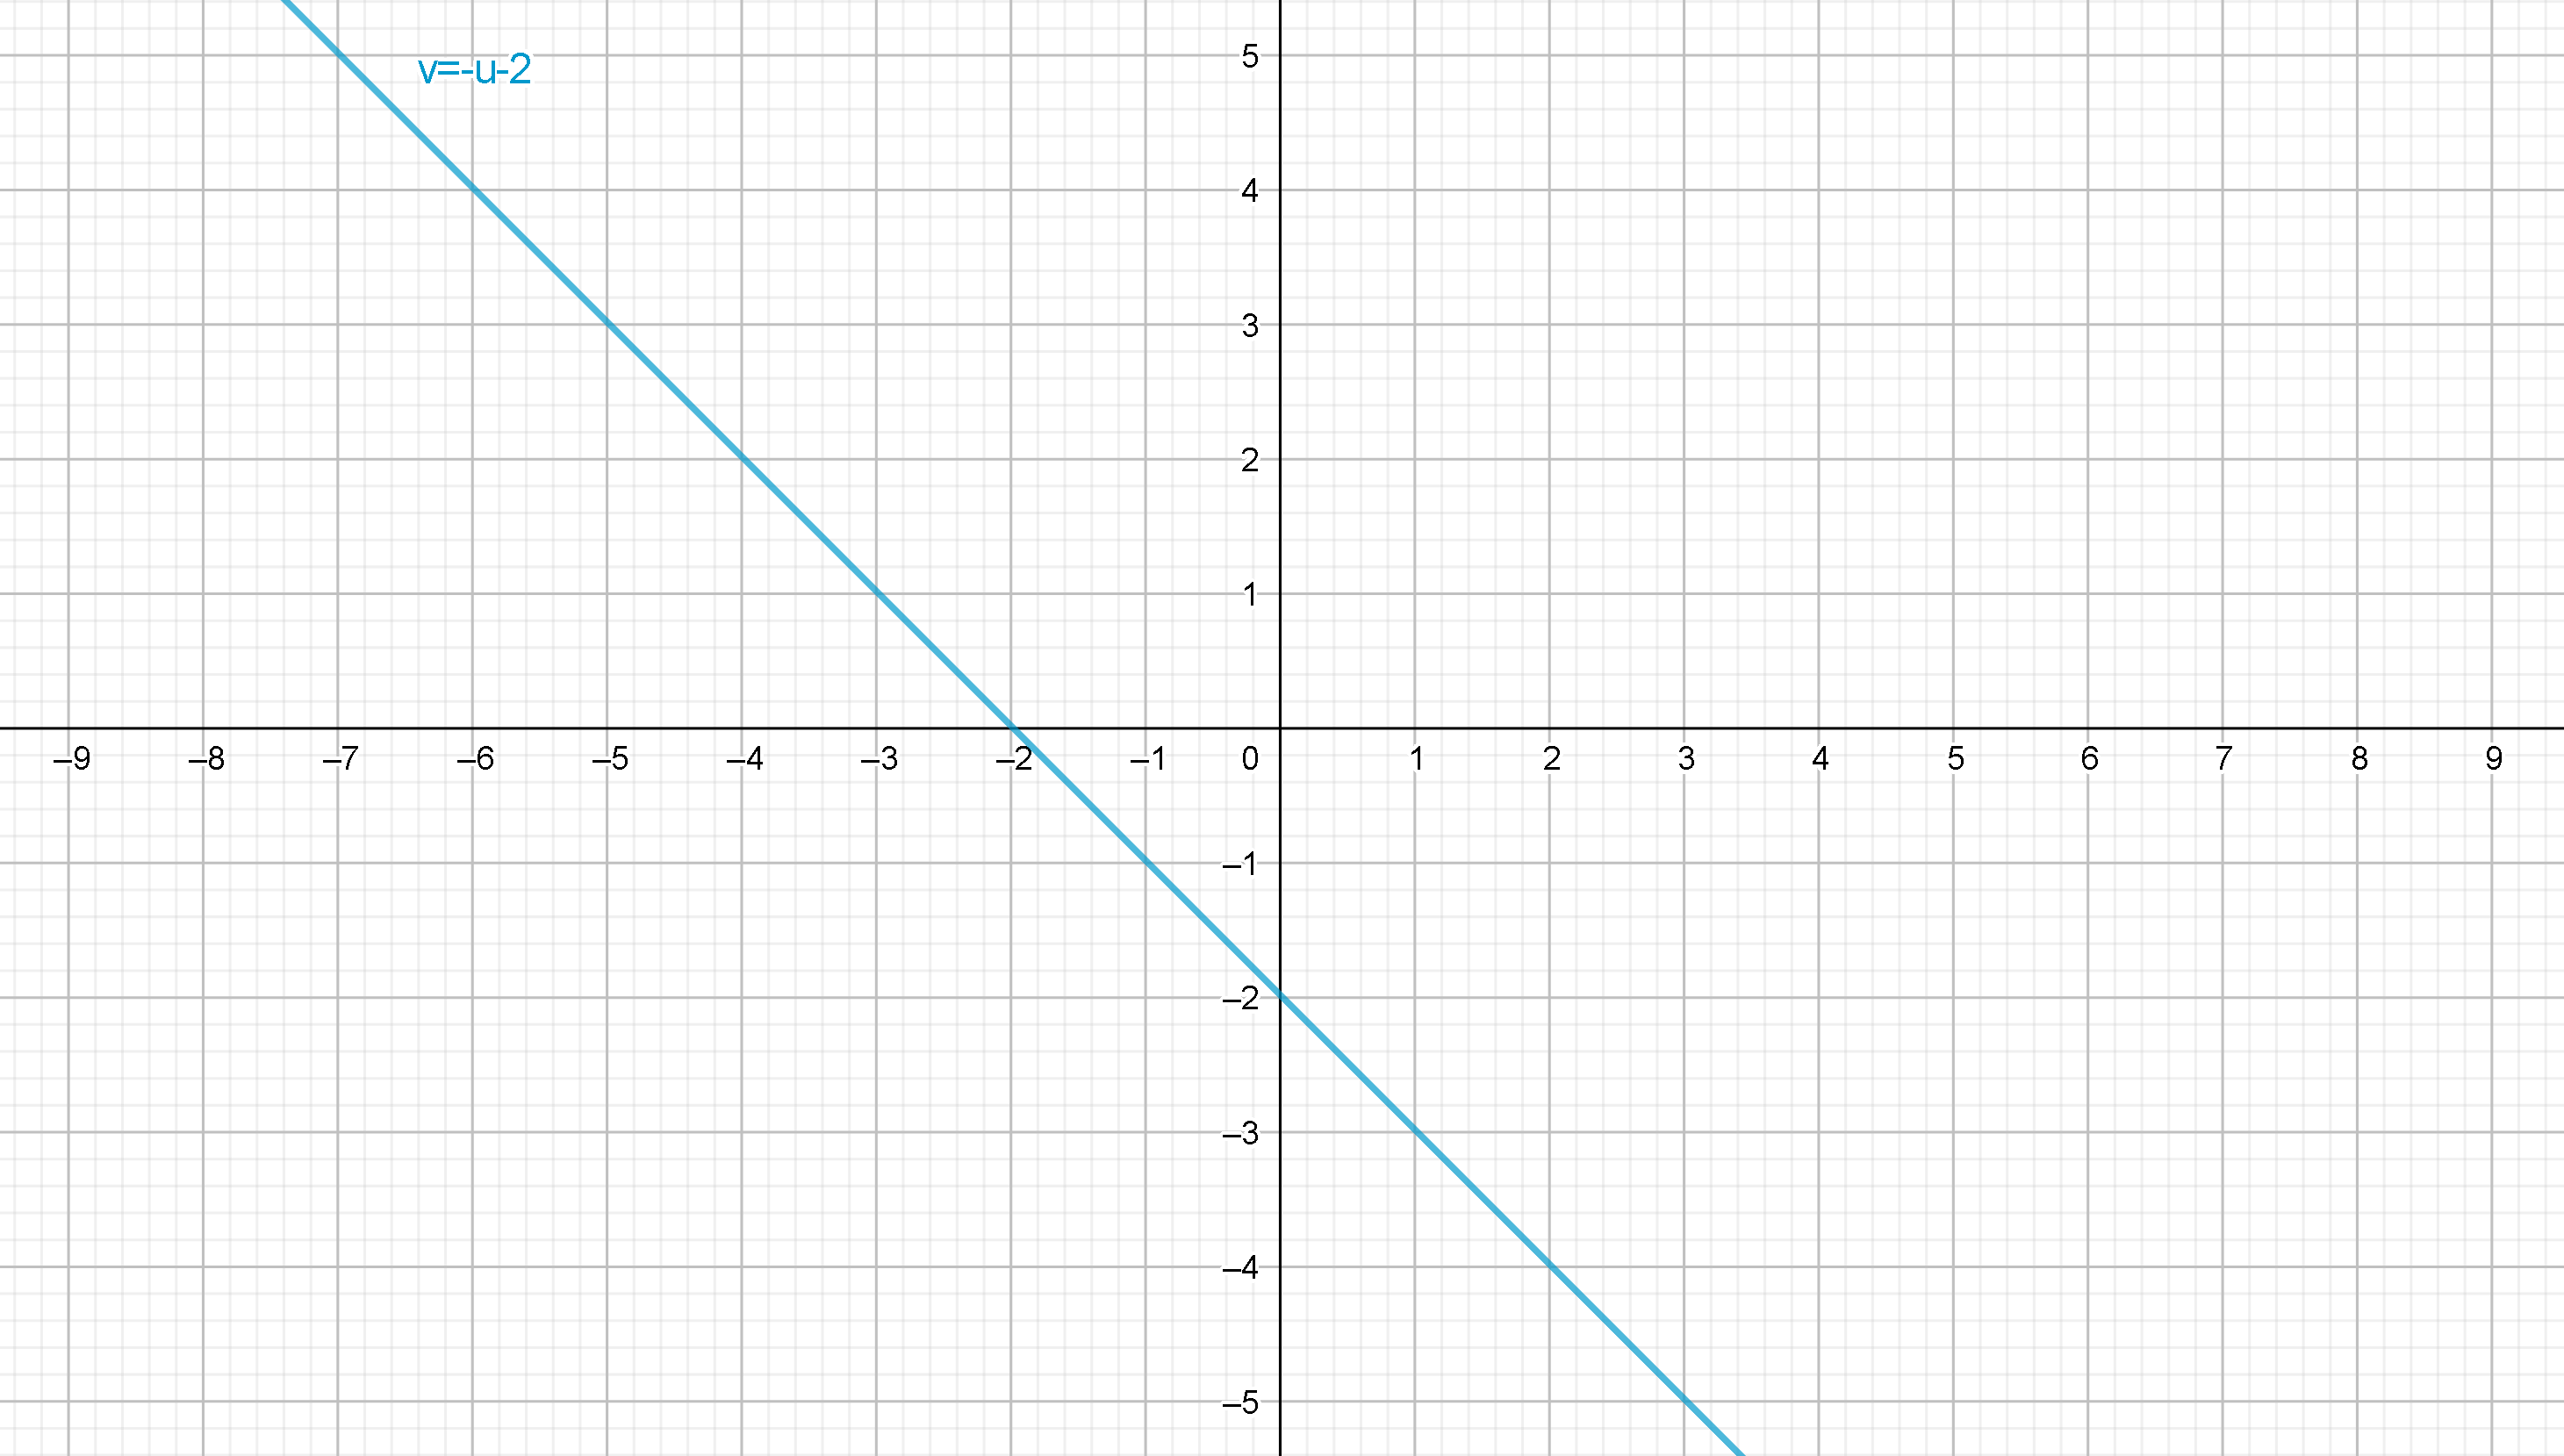
\includegraphics[width=11cm]{Mapeo Ej 1 w.png}
\end{center}

\textcolor{ao(english)}{\ding{46}} Punto de prueba.

$$z_{1}\,=\,5\,-\,4i$$

$$f(z_{1})\,=\,z_{1}\,+\,i\,(i\,-\,2)\,=\,5\,-\,4i\,+\,i\,(i\,-\,2)\,=\,5\,-\,4i\,-\,1\,-\,2\,i\,=\,4\,-\,6\,i$$


$$z_{2}\,=\,-\,3\,+\,4i$$

$$f(z_{2})\,=\,z_{2}\,+\,i\,(i\,-\,2)\,=\,-\,3\,+\,4i\,+\,i\,(i\,-\,2)\,=\,-\,3\,+\,4i\,-\,1\,-\,2\,i\,=\,-\,4\,+\,2\,i$$

\textcolor{ao(english)}{(\,2\,)} $\mathnormal{S}$ es $\boxed{\bf{1\,<\,\mathnormal{Re}(z)\,<\,4}}$ y $\boxed{\bf{f(z)\,=\,3\,z}}$.

$$f(z)\,=\,3\,z \iff 3\,x\,+\,3\,i\,y\, $$
$$ U\,=\,3\,x \quad V\,=\,3\,y\, $$
Despejando en terminos de x Y y
$$ x\,=\,\dfrac{U}{3} $$
$$ y\,=\,\dfrac{V}{3} $$
Remplazo x en S
$$ 1\,<\,x\,<\,4 \iff 1\,<\,\dfrac{U}{3}\,<\,4 $$
$$ 3\,<\,U\,<\,12 $$
Remplazo y segun S
$$ -\infty\,<\,y\,<\,\infty $$
$$ -\infty\,<\,\dfrac{V }{3}\,<\,\infty \iff -\infty\,<\,V\,<\,\infty$$

\newpage

\textcolor{ao(english)}{\ding{46}} Mapeo z-plano.

\begin{center}
     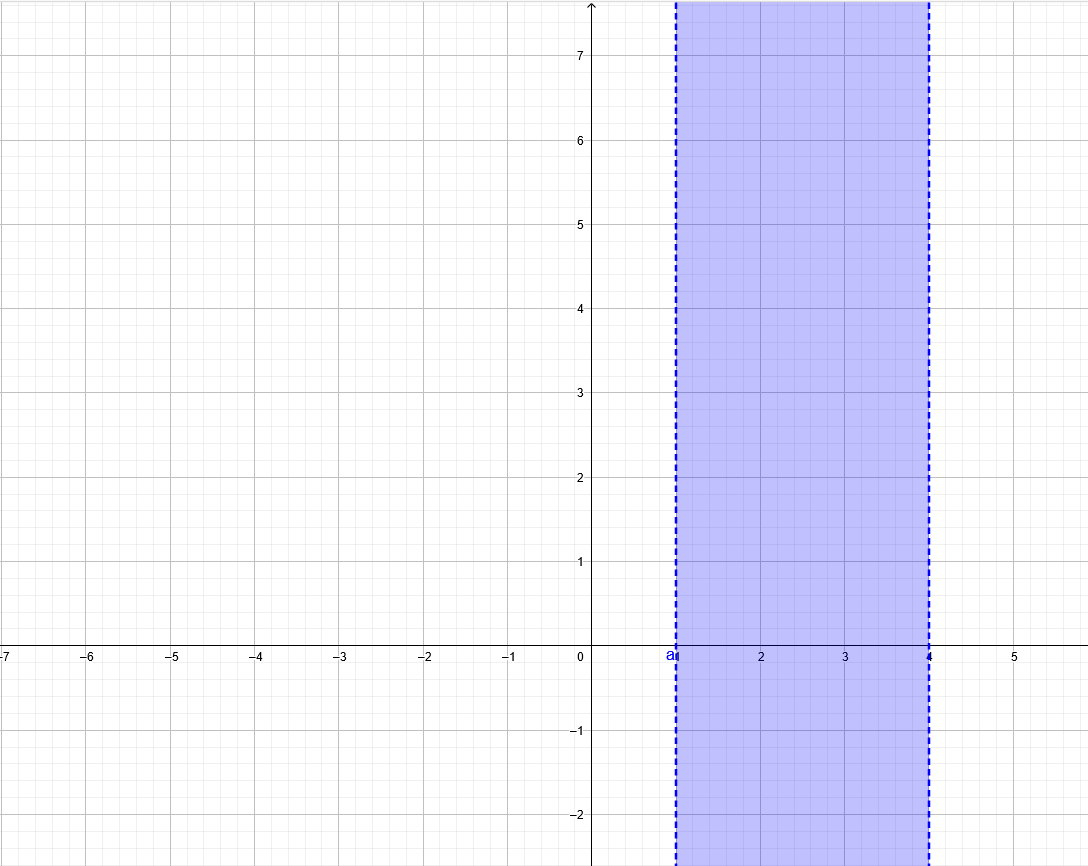
\includegraphics[width=10cm]{Mapeo-Ej-2-z}
\end{center}

\textcolor{ao(english)}{\ding{46}} Mapeo w-plano.

\begin{center}
     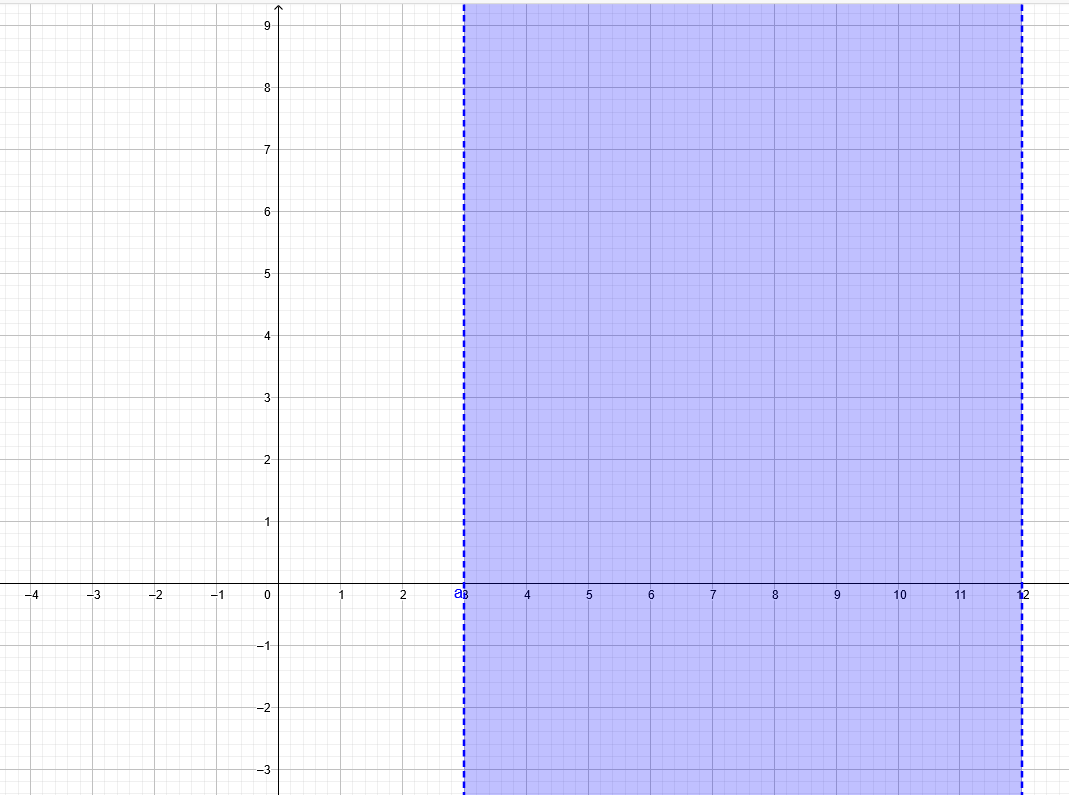
\includegraphics[width=10cm]{Mapeo-Ej-2-w}
\end{center}

\textcolor{ao(english)}{(\,3\,)} $\mathnormal{S}$ es $\boxed{\bf{y\,=\,-\,2}}$ y $\boxed{\bf{f(z)\,=\,2\,i\,+\,z\,(1\,+\,i)}}$.

\textcolor{ao(english)}{(\,4\,)} $\mathnormal{S}$ es $\boxed{\bf{-\,1\,<\,\mathnormal{Im}(z)\,<\,2}}$ y $\boxed{\bf{f(z)\,=\,i\,z\,+\,4}}$.

\textcolor{ao(english)}{(\,5\,)} $\mathnormal{S}$ es $\boxed{\bf{\mathnormal{Re}(z)\,>\,3}}$ y $\boxed{\bf{f(z)\,=\,z^{2}}}$.\\

\textcolor{ao(english)}{\ding{46}} Sustituir $z\,=\,x\,+\,i\,y$ en $E_{1}$.

$$\mathnormal{Re}(z)\,>\,3 \quad\iff\quad \mathnormal{Re}(x\,+\,i\,y)\,>\,3 \quad\iff\quad \underbrace{x\,>\,3}_{E_{1}}$$

\textcolor{ao(english)}{\ding{46}} Sustituir $z\,=\,x\,+\,i\,y$ en $f(z)$.

$$f(x\,+\,i\,y)\,=\,(x\,+\,i\,y)^{2}\,=\,x^{2}\,+\,2\,(x)\,(i\,y)\,+\,(i\,y)^{2}\,=\,x^{2}\,+\,i\,2\,x\,y\,-\,y^{2}$$

$$w\,=\,\underbrace{(x^{2}\,-\,y^{2})}_{u(x\,,\,y)}\,+\,i\,\underbrace{(2\,x\,y)}_{v(x\,,\,y)}$$

$$\underbrace{u\,=\,x^{2}\,-\,y^{2}}_{E_{2}} \qquad;\qquad \underbrace{v\,=\,2\,x\,y}_{E_{3}}$$

\textcolor{ao(english)}{\ding{46}} Sustituir $x\,=\,3$ en $E_{2}$ y despejar $y$.

$$u\,=\,\textcolor{ao}{3}^{2}\,-\,y^{2} \quad\iff\quad u\,=\,9\,-\,y^{2} \quad\iff\quad y^{2}\,=\,9\,-\,u \quad\iff\quad \underbrace{y\,=\,\sqrt{9\,-\,u}}_{E_{4}}$$

\textcolor{ao(english)}{\ding{46}} Despejar x en $E_{3}$ y sustituir en $E_{1}$.

$$v\,=\,2\,x\,y \quad\iff\quad x\,=\,\dfrac{v}{2\,y} \quad\iff\quad \textcolor{ao}{\dfrac{v}{2\,y}}\,>\,3 \quad\iff\quad \underbrace{v\,>\,6\,y}_{E_{5}}$$

\textcolor{ao(english)}{\ding{46}} Sustituir $E_{4}$ en $E_{5}$

$$v\,>\,6\,\textcolor{ao}{\sqrt{9\,-\,u}}$$

\textcolor{ao(english)}{\ding{46}} Punto de prueba.

$$z_{1}\,=\,5\,-\,4i$$

$$f(z_{1})\,=\,(z_{1})^{2}\,=\,(5\,-\,4i)^{2}\,=\,25\,-\,40\,i\,-\,16\,=\,9\,-\,40\,i$$


$$z_{2}\,=\,3\,+\,2i$$

$$f(z_{2})\,=\,(z_{2})^{2}\,=\,(3\,+\,2i)^{2}\,=\,9\,+\,12\,i\,-\,4\,=\,5\,+\,12\,i$$

\begin{center}
\textbf{Límites}
\end{center}

En los ejercicio \textbf{(\,6\,)} al \textbf{(\,11\,)} use las \textbf{propiedades de los límites} para calcular los límites indicados.\\

\textcolor{ao(english)}{(\,6\,)} $\bf{\displaystyle\lim_{z \to 2\,i}\,(z^{2}\,-\,\overline{z})}$

\textcolor{ao(english)}{(\,7\,)} $\bf{\displaystyle\lim_{z \to 3\,i}\,\dfrac{\mathnormal{Im}(z^{2})}{z\,+\,\mathnormal{Re}(z)}}$

$$\displaystyle\lim_{z \to 3\,i}\,\dfrac{\mathnormal{Im}(z^{2})}{z\,+\,\mathnormal{Re}(z)}\,=\,\dfrac{\mathnormal{Im}((3\,i)^{2})}{3\,i\,+\,\mathnormal{Re}(3\,i)}\,=\,\dfrac{\mathnormal{Im}(9\,i^{2})}{3\,i\,+\,0}\,=\,\dfrac{\mathnormal{Im}(-\,9)}{3\,i}\,=\,\dfrac{0}{3\,i}\,=\,0$$

\textcolor{ao(english)}{(\,8\,)} $\bf{\displaystyle\lim_{z \to 1\,+\,i}\,\dfrac{z^{2}\,+\,1}{z^{2}\,-\,1}}$

$$\dfrac{(\,1\,+\,i\,)^{2}\,+\,1}{(\,1\,+\,i)^{2}\,-\,1}$$

$$(\,1\,+\,i\,)^{2}\,=\,2\,i$$

$$\dfrac{\,2\,i\,\,+\,1}{\,2\,\,i\,-\,1} \times \dfrac{\,2\,i\,\,+\,1}{\,2\,\,i\,+\,1} $$

$$\dfrac{-\,4+\,2i\,\,+\,2i\,+\,1}{\,(2\,\,i)^{2}\,-\,1} \iff \dfrac{-\,3\,+\,4i\,}{\,-\,5} \iff \boxed{\dfrac{\,3\,}{\,\,5} - \dfrac{\,4i\,}{\,\,5}  }$$

\textcolor{ao(english)}{(\,9\,)} $\bf{\displaystyle\lim_{z \to 3\,+\,i\,\sqrt{2}}\,\dfrac{z\,+\,3\,-\,i\,\sqrt{2}}{z^{2}\,+\,6\,z\,+\,11}}$

\textcolor{ao(english)}{(\,10\,)} $\bf{\displaystyle\lim_{z \to 2}\,\dfrac{z\,2\,-\,5\,z\,+\,6}{z^{2}\,-\,4}}$

$$ \dfrac{\,2\,(2)\,-\,5\,(2)\,+\,6}{\,(2)^{2}\,-\,4} \iff \dfrac{\,4\,-\,10\,+\,6}{\,4\,-\,4} \iff \dfrac{0}{0}$$

Aplicando Hopital:

$$ f'\,(z_{0})\,= \displaystyle\lim_{z \to 2} \dfrac{\,2\,-\,5\,}{\,2\,(2)} \iff \dfrac{-\,3}{4} \iff \boxed{-\dfrac{3}{4}}$$

\textcolor{ao(english)}{(\,11\,)} $\bf{\displaystyle\lim_{z \to 3\,i}\,\dfrac{z^{4}\,+\,10\,z^{2}\,+\,9}{z^{2}\,-\,4\,i\,z\,-\,3}}$

$$\displaystyle\lim_{z \to 3\,i}\,\dfrac{z^{4}\,+\,10\,z^{2}\,+\,9}{z^{2}\,-\,4\,i\,z\,-\,3}\,=\,\dfrac{(3\,i)^{4}\,+\,10\,(3\,i)^{2}\,+\,9}{(3\,i)^{2}\,-\,4\,i\,(3\,i)\,-\,3}\,=\,\dfrac{81\,i^{4}\,+\,90\,i^{2}\,+\,9}{9\,i^{2}\,-\,12\,i^{2}\,-\,3}$$

$$=\,\dfrac{81\,-\,90\,+\,9}{-\,9\,+\,12\,-\,3}\,=\,\dfrac{90\,-\,90}{12\,-\,12}\,=\,\dfrac{0}{0}$$

\textcolor{ao(english)}{\ding{46}} Usamos la regla de L'Hopital.

\definecolor{britishracinggreen}{rgb}{0.0, 0.26, 0.15}

$$=\,\displaystyle\lim_{z \to 3\,i}\,\dfrac{4\,z^{3}\,+\,20\,z}{2\,z\,-\,4\,i}\,=\,\dfrac{4\,(3\,i)^{3}\,+\,20\,(3\,i)}{2\,(3\,i)\,-\,4\,i}\,=\,\dfrac{4\,(-\,27\,i)\,+\,60\,i}{6\,i\,-\,4\,i}\,=\,\dfrac{-\,108\,i\,+\,60\,i}{2\,i}\,=\,\dfrac{-\,48\,i}{2\,i}$$

$$=\,\dfrac{-\,48\,i}{2\,i}\,\textcolor{britishracinggreen}{\times\,\dfrac{-\,2\,i}{-\,2\,i}}\,=\,\dfrac{96\,i^{2}}{-\,2\,i^{2}}\,=\,\dfrac{-\,96}{2}\,=\,-\,48$$

\begin{center}
\textbf{Derivadas}
\end{center}

\textcolor{ao(english)}{(\,12\,)} Use la fórmula de la \textbf{Definición de Derivada} mostrada a continuación:\\

$$\bf{f\,'\,(z_{0})\,=\,\displaystyle\lim_{\Delta\,z \to 0}\,\dfrac{f(z_{0}\,+\,\Delta\,z)\,-\,f(z_{0})}{\Delta\,z}}$$\\

para calcular la derivada de la función $\bf{f(z)\,=\,z\,\mathnormal{Im}(z)}$ en los puntos $\bf{z_{0}\,=\,0}$, $\bf{z_{0}\,=\,1\,+\,i}$ y $\bf{z_{0}\,=\,-\,2\,-\,i}$. ¿Ésta función es Analítica?\\

\begin{tcolorbox}[colback=ao(english)!5!white,colframe=ao(english)!75!black,fonttitle=\bfseries,title=\sf Recordemos que:]

\textcolor{ao(english)}{\ding{42}} $z_{0}\,=\,0 \quad\iff\quad z_{0}\,=\,0\,+\,0\,i$.\\

\textcolor{ao(english)}{\ding{42}} $\Delta\,z\,=\,\Delta\,x\,+\,i\,\Delta\,y$

\end{tcolorbox}

\definecolor{cadmiumgreen}{rgb}{0.0, 0.42, 0.24}

\textcolor{ao(english)}{\ding{46}} Calcular la derivada del punto $z_{0}\,=\,0$.\\

\textcolor{ao(english)}{\ding{47}} Construir $f(z_{0}\,+\,\Delta\,z)$ y $f(z_{0})$.

$$f(z_{0}\,+\,\Delta\,z)\,=\,(z_{0}\,+\,\Delta\,z)\,\mathnormal{Im}(z_{0}\,+\,\Delta\,z)\,=\,(0\,+\,0\,i\,+\,\Delta\,x\,+\,i\,\Delta\,y)\,\mathnormal{Im}(0\,+\,0\,i\,+\,\Delta\,x\,+\,i\,\Delta\,y)$$

$$=\,\left[(0\,+\,\Delta\,x)\,+\,i(0\,+\,\Delta\,y)\right]\,\mathnormal{Im}\left[(0\,+\,\Delta\,x)\,+\,i(0\,+\,\Delta\,y)\right]\,=\,(\Delta\,x\,+\,i\Delta\,y)\,\mathnormal{Im}(\Delta\,x\,+\,i\Delta\,y)$$

$$f(z_{0}\,+\,\Delta\,z)\,=\,\Delta\,y\,(\Delta\,x\,+\,i\,\Delta\,y)$$

$$f(z_{0})\,=\,z_{0}\,\mathnormal{Im}(z_{0})\,=\,(0\,+\,0\,i)\,\mathnormal{Im}(0\,+\,0\,i)\,=\,(0\,+\,0\,i)\,0\,=\,0$$

\textcolor{ao(english)}{\ding{47}} Sustituir  $f(z_{0}\,+\,\Delta\,z)$ y $f(z_{0})$ en la defición de Derivadas.

$$f\,'\,(z_{0})\,=\,\displaystyle\lim_{\Delta\,z \to 0}\,\dfrac{\Delta\,y\,(\Delta\,x\,+\,i\,\Delta\,y)\,-\,0}{\Delta\,x\,+\,i\,\Delta\,y}\,=\,\displaystyle\lim_{\Delta\,z \to 0}\,\dfrac{\Delta\,y\,(\Delta\,x\,+\,i\Delta\,y)}{\Delta\,x\,+\,i\,\Delta\,y}$$

\textcolor{ao(english)}{\ding{47}} Trayectoria $\parallel$ eje $x \quad\Rightarrow\quad \Delta\,y\,=\,0$

$$f\,'\,(z_{0})\,=\,\displaystyle\lim_{\Delta\,x \to 0}\,\dfrac{0\,(\Delta\,x\,+\,0\,i)}{\Delta\,x\,+\,0\,i}\,=\,\displaystyle\lim_{\Delta\,x \to 0}\,\dfrac{0}{\Delta\,x}\,=\,\displaystyle\lim_{\Delta\,x \to 0}\,0\,=\,0$$

$$L_{1}\,=\,0$$

\textcolor{ao(english)}{\ding{47}} Trayectoria $\parallel$ eje $y \quad\Rightarrow\quad \Delta\,x\,=\,0$

$$f\,'\,(z_{0})\,=\,\displaystyle\lim_{\Delta\,y \to 0}\,\dfrac{\Delta\,y\,(0\,+\,i\Delta\,y)}{0\,+\,i\,\Delta\,y}\,=\,\displaystyle\lim_{\Delta\,y \to 0}\,\dfrac{i\,(\Delta\,y)^{\cancel{2}}}{i\,\cancel{\Delta\,y}}\,=\,\displaystyle\lim_{\Delta\,y \to 0}\,\dfrac{i\,\Delta\,y}{i}\,=\,\dfrac{0\,i}{i}\,=\,0$$

$$L_{2}\,=\,0$$

\textcolor{ao(english)}{\ding{46}} Calcular la derivada del punto $z_{0}\,=\,1\,+\,i$.\\

\textcolor{ao(english)}{\ding{47}} Construir $f(z_{0}\,+\,\Delta\,z)$ y $f(z_{0})$.

$$f(z_{0}\,+\,\Delta\,z)\,=\,(z_{0}\,+\,\Delta\,z)\,\mathnormal{Im}(z_{0}\,+\,\Delta\,z)\,=\,(1\,+\,i\,+\,\Delta\,x\,+\,i\,\Delta\,y)\,\mathnormal{Im}(1\,+\,i\,+\,\Delta\,x\,+\,i\,\Delta\,y)$$

$$=\,\left[(1\,+\,\Delta\,x)\,+\,i(1\,+\,\Delta\,y)\right]\,\mathnormal{Im}\left[(1\,+\,\Delta\,x)\,+\,i(1\,+\,\Delta\,y)\right]\,=\,\left[(1\,+\,\Delta\,x)\,+\,i(1\,+\,\Delta\,y)\right]\,(1\,+\,\Delta\,y)$$

$$f(z_{0}\,+\,\Delta\,z)\,=\,(1\,+\,\Delta\,y)\,\left[(1\,+\,\Delta\,x)\,+\,i(1\,+\,\Delta\,y)\right]$$

$$f(z_{0})\,=\,z_{0}\,\mathnormal{Im}(z_{0})\,=\,(1\,+\,i)\,\mathnormal{Im}(1\,+\,i)\,=\,1\,+\,i$$

$$f(z_{0})\,=\,1\,+\,i$$

\textcolor{ao(english)}{\ding{47}} Sustituir  $f(z_{0}\,+\,\Delta\,z)$ y $f(z_{0})$ en la defición de Derivadas.

$$f\,'\,(z_{0})\,=\,\displaystyle\lim_{\Delta\,z \to 0}\,\dfrac{(1\,+\,\Delta\,y)\,\left[(1\,+\,\Delta\,x)\,+\,i\,(1\,+\,\Delta\,y)\right]\,-\,(1\,+\,i)}{\Delta\,x\,+\,i\,\Delta\,y}$$

$$f\,'\,(z_{0})\,=\,\displaystyle\lim_{\Delta\,z \to 0}\,\dfrac{(1\,+\,\Delta\,y)\,\left[(1\,+\,\Delta\,x)\,+\,i\,(1\,+\,\Delta\,y)\right]\,-\,1\,-\,i}{\Delta\,x\,+\,i\,\Delta\,y}$$

\textcolor{ao(english)}{\ding{47}} Trayectoria $\parallel$ eje $x \quad\Rightarrow\quad \Delta\,y\,=\,0$

$$f\,'\,(z_{0})\,=\,\displaystyle\lim_{\Delta\,x \to 0}\,\dfrac{(1\,+\,0)\,\left[(1\,+\,\Delta\,x)\,+\,i\,(1\,+\,0)\right]\,-\,1\,-\,i}{\Delta\,x\,+\,0\,i}\,=\,\displaystyle\lim_{\Delta\,x \to 0}\,\dfrac{1\,+\,\Delta\,x\,+\,i\,-\,1\,-\,i}{\Delta\,x}$$

$$=\,\displaystyle\lim_{\Delta\,x \to 0}\,\dfrac{\Delta\,x}{\Delta\,x}\,=\,\displaystyle\lim_{\Delta\,x \to 0}\,1\,=\,1$$

$$L_{1}\,=\,1$$

\textcolor{ao(english)}{\ding{47}} Trayectoria $\parallel$ eje $y \quad\Rightarrow\quad \Delta\,x\,=\,0$

$$f\,'\,(z_{0})\,=\,\displaystyle\lim_{\Delta\,y \to 0}\,\dfrac{(1\,+\,\Delta\,y)\,\left[(1\,+\,0)\,+\,i\,(1\,+\,\Delta\,y)\right]\,-\,1\,-\,i}{0\,+\,i\,\Delta\,y}$$

$$=\,\displaystyle\lim_{\Delta\,y \to 0}\,\dfrac{(1\,+\,\Delta\,y)\,\left[1\,+\,i\,(1\,+\,\Delta\,y)\right]\,-\,1\,-\,i}{i\,\Delta\,y}\,=\,\displaystyle\lim_{\Delta\,y \to 0}\,\dfrac{1\,+\,\Delta\,y\,+\,i\,(1\,+\,\Delta\,y)^{2}\,-\,1\,-\,i}{i\,\Delta\,y}$$

$$=\,\displaystyle\lim_{\Delta\,y \to 0}\,\dfrac{\Delta\,y\,+\,i[1\,+\,2\,\Delta\,y\,+\,(\Delta\,y)^{2}]\,-\,i}{i\,\Delta\,y}\,=\,\displaystyle\lim_{\Delta\,y \to 0}\,\dfrac{\Delta\,y\,+\,i\,+\,2\,i\,\Delta\,y\,+\,i\,(\Delta\,y)^{2}\,-\,i}{i\,\Delta\,y}$$

$$=\,\displaystyle\lim_{\Delta\,y \to 0}\,\dfrac{\cancel{\Delta\,y}\,+\,2\,i\,\cancel{\Delta\,y}\,+\,i\,(\Delta\,y)^{\cancel{2}}}{i\,\cancel{\Delta\,y}}\,=\,\displaystyle\lim_{\Delta\,y \to 0}\,\dfrac{1\,+\,2\,i\,\,+\,i\,\Delta\,y}{i}\,=\,\displaystyle\lim_{\Delta\,y \to 0}\,\dfrac{1\,+\,i\,(2\,\,+\,\Delta\,y)}{i}$$

$$=\,\dfrac{1\,+\,i\,(2\,\,+\,0)}{i}\,=\,\dfrac{1\,+\,2\,i}{i}$$

$$L_{2}\,=\,\dfrac{1\,+\,2\,i}{i}\,\textcolor{cadmiumgreen}{\times\,\dfrac{-\,i}{-\,i}}\,=\,\dfrac{-\,i\,-\,2\,i^{2}}{-\,i^{2}}\,=\,2\,-\,i$$

\textcolor{ao(english)}{\ding{46}} Calcular la derivada del punto $z_{0}\,=\,-\,2\,-\,i$.\\

\textcolor{ao(english)}{\ding{47}} Construir $f(z_{0}\,+\,\Delta\,z)$ y $f(z_{0})$.

$$f(z_{0}\,+\,\Delta\,z)\,=\,(z_{0}\,+\,\Delta\,z)\,\mathnormal{Im}(z_{0}\,+\,\Delta\,z)\,=\,(-\,2\,-\,i\,+\,\Delta\,x\,+\,i\,\Delta\,y)\,\mathnormal{Im}(-\,2\,-\,i\,+\,\Delta\,x\,+\,i\,\Delta\,y)$$

$$=\,\left[(-\,2\,+\,\Delta\,x)\,+\,i(-\,1\,+\,\Delta\,y)\right]\,\mathnormal{Im}\left[(-\,2\,+\,\Delta\,x)\,+\,i(-\,1\,+\,\Delta\,y)\right]$$

$$=\,\left[(-\,2\,+\,\Delta\,x)\,+\,i(-\,1\,+\,\Delta\,y)\right]\,(-\,1\,+\,\Delta\,y)$$

$$f(z_{0}\,+\,\Delta\,z)\,=\,(-\,1\,+\,\Delta\,y)\,\left[(-\,2\,+\,\Delta\,x)\,+\,i(-\,1\,+\,\Delta\,y)\right]$$

$$f(z_{0})\,=\,z_{0}\,\mathnormal{Im}(z_{0})\,=\,(-\,2\,-\,i)\,\mathnormal{Im}(-\,2\,-\,i)\,=\,(-\,2\,-\,i)\,(-\,1)$$

$$f(z_{0})\,=\,2\,+\,i$$

\textcolor{ao(english)}{\ding{47}} Sustituir  $f(z_{0}\,+\,\Delta\,z)$ y $f(z_{0})$ en la defición de Derivadas.

$$f\,'\,(z_{0})\,=\,\displaystyle\lim_{\Delta\,z \to 0}\,\dfrac{(-\,1\,+\,\Delta\,y)\,\left[(-\,2\,+\,\Delta\,x)\,+\,i\,(-\,1\,+\,\Delta\,y)\right]\,-\,(2\,+\,i)}{\Delta\,x\,+\,i\,\Delta\,y}$$

$$f\,'\,(z_{0})\,=\,\displaystyle\lim_{\Delta\,z \to 0}\,\dfrac{(-\,1\,+\,\Delta\,y)\,\left[(-\,2\,+\,\Delta\,x)\,+\,i\,(-\,1\,+\,\Delta\,y)\right]\,-\,2\,-\,i}{\Delta\,x\,+\,i\,\Delta\,y}$$

\textcolor{ao(english)}{\ding{47}} Trayectoria $\parallel$ eje $x \quad\Rightarrow\quad \Delta\,y\,=\,0$

$$f\,'\,(z_{0})\,=\,\displaystyle\lim_{\Delta\,x \to 0}\,\dfrac{(-\,1\,+\,0)\,\left[(-\,2\,+\,\Delta\,x)\,+\,i\,(-\,1\,+\,0)\right]\,-\,2\,-\,i}{\Delta\,x\,+\,0\,i}$$

$$=\,\displaystyle\lim_{\Delta\,x \to 0}\,\dfrac{(-\,1)\,\left[(-\,2\,+\,\Delta\,x)\,-\,i\right]-\,2\,-\,i}{\Delta\,x\,+\,0\,i}\,=\,\displaystyle\lim_{\Delta\,x \to 0}\,\dfrac{(-\,1)\,(-\,2\,+\,\Delta\,x)\,+\,i\,-\,2\,-\,i}{\Delta\,x}$$

$$=\,\displaystyle\lim_{\Delta\,x \to 0}\,\dfrac{2\,-\,\Delta\,x\,-\,2}{\Delta\,x}\,=\,\displaystyle\lim_{\Delta\,x \to 0}\,\dfrac{-\,\Delta\,x}{\Delta\,x}\,=\,\displaystyle\lim_{\Delta\,x \to 0}\,-\,1\,=\,-\,1$$

$$L_{1}\,=\,-\,1$$

\textcolor{ao(english)}{\ding{47}} Trayectoria $\parallel$ eje $y \quad\Rightarrow\quad \Delta\,x\,=\,0$

$$f\,'\,(z_{0})\,=\,\displaystyle\lim_{\Delta\,y \to 0}\,\dfrac{(-\,1\,+\,\Delta\,y)\,\left[(-\,2\,+\,0)\,+\,i\,(-\,1\,+\,\Delta\,y)\right]\,-\,2\,-\,i}{0\,+\,i\,\Delta\,y}$$

$$=\,\displaystyle\lim_{\Delta\,y \to 0}\,\dfrac{2\,-\,2\,\Delta\,y\,+\,i\,(-\,1\,+\,\Delta\,y)^{2}\,-\,2\,-\,i}{i\,\Delta\,y}\,=\,\displaystyle\lim_{\Delta\,y \to 0}\,\dfrac{-\,2\,\Delta\,y\,+\,i\,(-\,1\,+\,\Delta\,y)^{2}\,-\,i}{i\,\Delta\,y}$$

$$=\,\displaystyle\lim_{\Delta\,y \to 0}\,\dfrac{-\,2\,\Delta\,y\,+\,i\,[1\,-\,2\,\Delta\,y\,+\,(\Delta\,y)^{2}]\,-\,i}{i\,\Delta\,y}\,=\,\displaystyle\lim_{\Delta\,y \to 0}\,\dfrac{-\,2\,\Delta\,y\,+\,i\,-\,2\,i\,\Delta\,y\,+\,i\,(\Delta\,y)^{2}\,-\,i}{i\,\Delta\,y}$$

$$=\,\displaystyle\lim_{\Delta\,y \to 0}\,\dfrac{-\,2\,\cancel{\Delta\,y}\,-\,2\,i\,\cancel{\Delta\,y}\,+\,i\,(\Delta\,y)^{\cancel{2}}}{i\,\cancel{\Delta\,y}}\,=\,\displaystyle\lim_{\Delta\,y \to 0}\,\dfrac{-\,2\,-\,2\,i\,+\,i\,\Delta\,y}{i}\,=\,\displaystyle\lim_{\Delta\,y \to 0}\,\dfrac{-\,2\,+\,i\,(-\,2\,+\,\Delta\,y)}{i}$$

$$=\,\dfrac{-\,2\,+\,i\,(-\,2\,+\,0)}{i}\,=\,\dfrac{-\,2\,-\,2\,i}{i}$$

$$L_{2}\,=\,\dfrac{-\,2\,-\,2\,i}{i}\,\textcolor{cadmiumgreen}{\times\,\dfrac{-\,i}{-\,i}}\,=\,\dfrac{2\,i\,+\,2\,i^{2}}{-\,i^{2}}\,=\,-\,2\,+\,2\,i$$

\textcolor{ao(english)}{\ding{46}} Conclusión:\\

La función $f(z)\,=\,z\,\mathnormal{Im}(z)$ no es una función analítica, porque los puntos $z_{0}\,=\,1\,+\,i$ y $z_{0}\,=\,-\,2\,-\,i$ sus límites $L_{1}\,\neq\,L_{2}$ tomando 2 trayectorias diferentes; entonces no existe límite o derivada para los puntos anteriormente mecionados. Pero para el punto $z_{0}\,=\,0$ su límites $L_{1}\,=\,L_{2}$ tomando 2 trayectorias diferentes; demuestra que exite límete unicamente en ese punto, por lo tanto tambien existe la derivada en dicho punto.\\

En los ejercicio \textbf{(\,13\,)} al \textbf{(\,15\,)} derive las siguientes funciones usando las \textbf{Reglas de la diferencición} (simplifique tanto como sea posible).\\

\textcolor{ao(english)}{(\,13\,)} $\bf{f(z)\,=\,-\,5\,z^{2}\,+\,\dfrac{2\,+\,i}{z^{2}}}$

$$f(z)\,=\,-\,5\,z^{2}\,+\,(2\,+\,i)\,z^{-\,2}$$

$$f\,'(z)\,=\,-\,5\,(2\,z)\,+\,(2\,+\,i)\,(-\,2\,z^{-\,3})\,=\,-\,10\,z\,-\,2\,(2\,+\,i)\,z^{-\,3}$$

$$f\,'(z)\,=\,-\,10\,z\,-\,\dfrac{4\,+\,2\,i}{z^{3}}$$

\textcolor{ao(english)}{(\,14\,)} $\bf{f(z)\,=\,(i\,z^{2}\,+\,3\,z)^{5}}$

$$ \boxed{f'\,(z)\,= 5(i\,z^{2}\,+\,3\,z)^{4} \cdot (\,2\,i\,z\,+\,3\,)} $$

\textcolor{ao(english)}{(\,15\,)} $\bf{f(z)\,=\,(z^{2}\,+\,2\,z\,-\,7\,i)^{2}\,(z^{4}\,-\,4\,i\,z)^{3}}$

\begin{center}
\textbf{Ecuaciones de Cauchy-Riemann}
\end{center}

En los ejercicio \textbf{(\,16\,)} al \textbf{(\,20\,)}, use las Ecuaciones de Cauchy-Riemann para mostrar si las siguientes funciones complejas son o no Analíticas.

\textcolor{ao(english)}{(\,16\,)} $\bf{f(z)\,=\,z^{2}\,+\,5\,i\,z\,+\,3\,-\,i}$

\textcolor{ao(english)}{(\,17\,)} $\bf{f(z)\,=\,e^{2\,x}\,(\cos\,y\,+\,i\,\sin\,y)}$

$$f(z)\,=\,e^{2\,x}\,\cos\,y\,+\,i\,e^{2\,x}\,\sin\,y$$

$$u\,=\,e^{2\,x}\,\cos\,y \quad;\quad v\,=\,e^{2\,x}\,\sin\,y$$

\textcolor{ao(english)}{\ding{46}} Usamos la ecuaciones de C-R.

$$\dfrac{\partial\,u}{\partial\,x}\,=\,e^{2\,x}\,\cos\,y\,=\,2\,e^{2\,x}\,\cos\,y$$

$$\dfrac{\partial\,v}{\partial\,y}\,=\,e^{2\,x}\,\sin\,y\,=\,e^{2\,x}\,\cos\,y$$

$$\dfrac{\partial\,u}{\partial\,x}\,\neq\,\dfrac{\partial\,v}{\partial\,y}$$

$\therefore$ la función no es analítica.\\

\textcolor{ao(english)}{(\,18\,)} $\bf{f(z)\,=\,3\,z^{2}\,+\,5\,z\,-\,6\,i}$

$$f(z)\,=\,3\,(x\,+\,i\,y)^{2}\,+\,5\,(x\,-\,i\,y)\,-\,6\,i\,\iff 3\,(x^{2}\,+\,2\,i\,x\,y\,-\,y^{2})\,+\,5\,(x\,-\,i\,y)\,-\,6\,i\, $$  

$$f(z)\,= \,3\,x^{2}\,+\,6\,i\,x\,y\,-\,3\,y^{2}\,+\,5\,x\,+\,5\,i\,y\,-\,6\,i$$

$$u\,=\,3\,x^{2}+\,5\,x-\,3\,y^{2} \quad;\quad v\,=\,6\,\,x\,y\,+\,5\,\,y-\,6\,$$

\textcolor{ao(english)}{\ding{46}} Usamos la ecuaciones de C-R.

$$\dfrac{\partial\,u}{\partial\,x}\,=\,6\,x\,+\,5$$

$$\dfrac{\partial\,v}{\partial\,y}\,=\,6\,x\,+\,5$$

$$\dfrac{\partial\,u}{\partial\,y}\,=\,-6\,y$$

$$-\dfrac{\partial\,v}{\partial\,x}\,=\,6\,y$$

$$\dfrac{\partial\,v}{\partial\,x}\,=-\,6\,y$$

La función es analítica.\\

\textcolor{ao(english)}{(\,19\,)} $\bf{f(z)\,=\,4\,z\,-\,6\,\overline{z}\,+\,3}$

$$f(x\,+\,i\,y)\,=\,4\,(x\,+\,i\,y)\,-\,6\,(x\,-\,i\,y)\,+\,3\,=\,4\,x\,+\,4\,i\,y\,-\,6\,x\,+\,6\,i\,y\,+\,3,=\,-\,2\,x\,+\,10\,i\,y\,+\,3$$

$$f(x\,+\,i\,y)\,=\,(3\,-\,2\,x)\,+\,10\,i\,y$$

$$u\,=\,3\,-\,2\,x \quad;\quad v\,=\,10\,y$$

\textcolor{ao(english)}{\ding{46}} Usamos la ecuaciones de C-R.

$$\dfrac{\partial\,u}{\partial\,x}\,=\,3\,-\,2\,x\,=\,-\,2$$

$$\dfrac{\partial\,v}{\partial\,y}\,=\,10\,y\,=\,10$$

$$\dfrac{\partial\,u}{\partial\,x}\,\neq\,\dfrac{\partial\,v}{\partial\,y}$$

$\therefore$ la función no es analítica.\\

\textcolor{ao(english)}{(\,20\,)} $\bf{f(z)\,=\,e^{-\,x}\,(\cos\,y\,-\,i\,\sin\,y)}$

$$u\,=\,e^{-\,x}\cos\,y \quad;\quad v\,=\,-e^{-\,x}\,i\,\sin\,y$$

\textcolor{ao(english)}{\ding{46}} Usamos la ecuaciones de C-R.

$$\dfrac{\partial\,u}{\partial\,x}\,=\,e^{-\,x}\cos\,y$$

$$\dfrac{\partial\,v}{\partial\,y}\,=\,-e^{-\,x}\,\cos\,y$$

$$\dfrac{\partial\,u}{\partial\,x}\,\neq\,\dfrac{\partial\,v}{\partial\,y}$$

La función no es analítica.\\

\end{document}